\documentclass{article}
\usepackage{graphicx} % Required for inserting images
\usepackage{geometry}
\usepackage{circuitikz}
\usepackage{siunitx}
\usepackage{CJKutf8}
\usepackage{amsmath}
\usepackage{amssymb}
\usepackage{caption}
\usepackage{float}
\usepackage{subcaption}
\geometry{top=5mm, left=30mm, a4paper}




\title{Integrator and Differentiator Report}
\author{梁程捷 (B11901136), 吳奕娃 (B11901080)}
\date{}


\begin{document}
\begin{CJK*}{UTF8}{bkai}
\maketitle
%=========Inverting OP-Amp Circuit=================
\section{Integrator}



\begin{figure}[h]
\begin{center}

    \begin{subfigure}[b]{0.2\textwidth}
        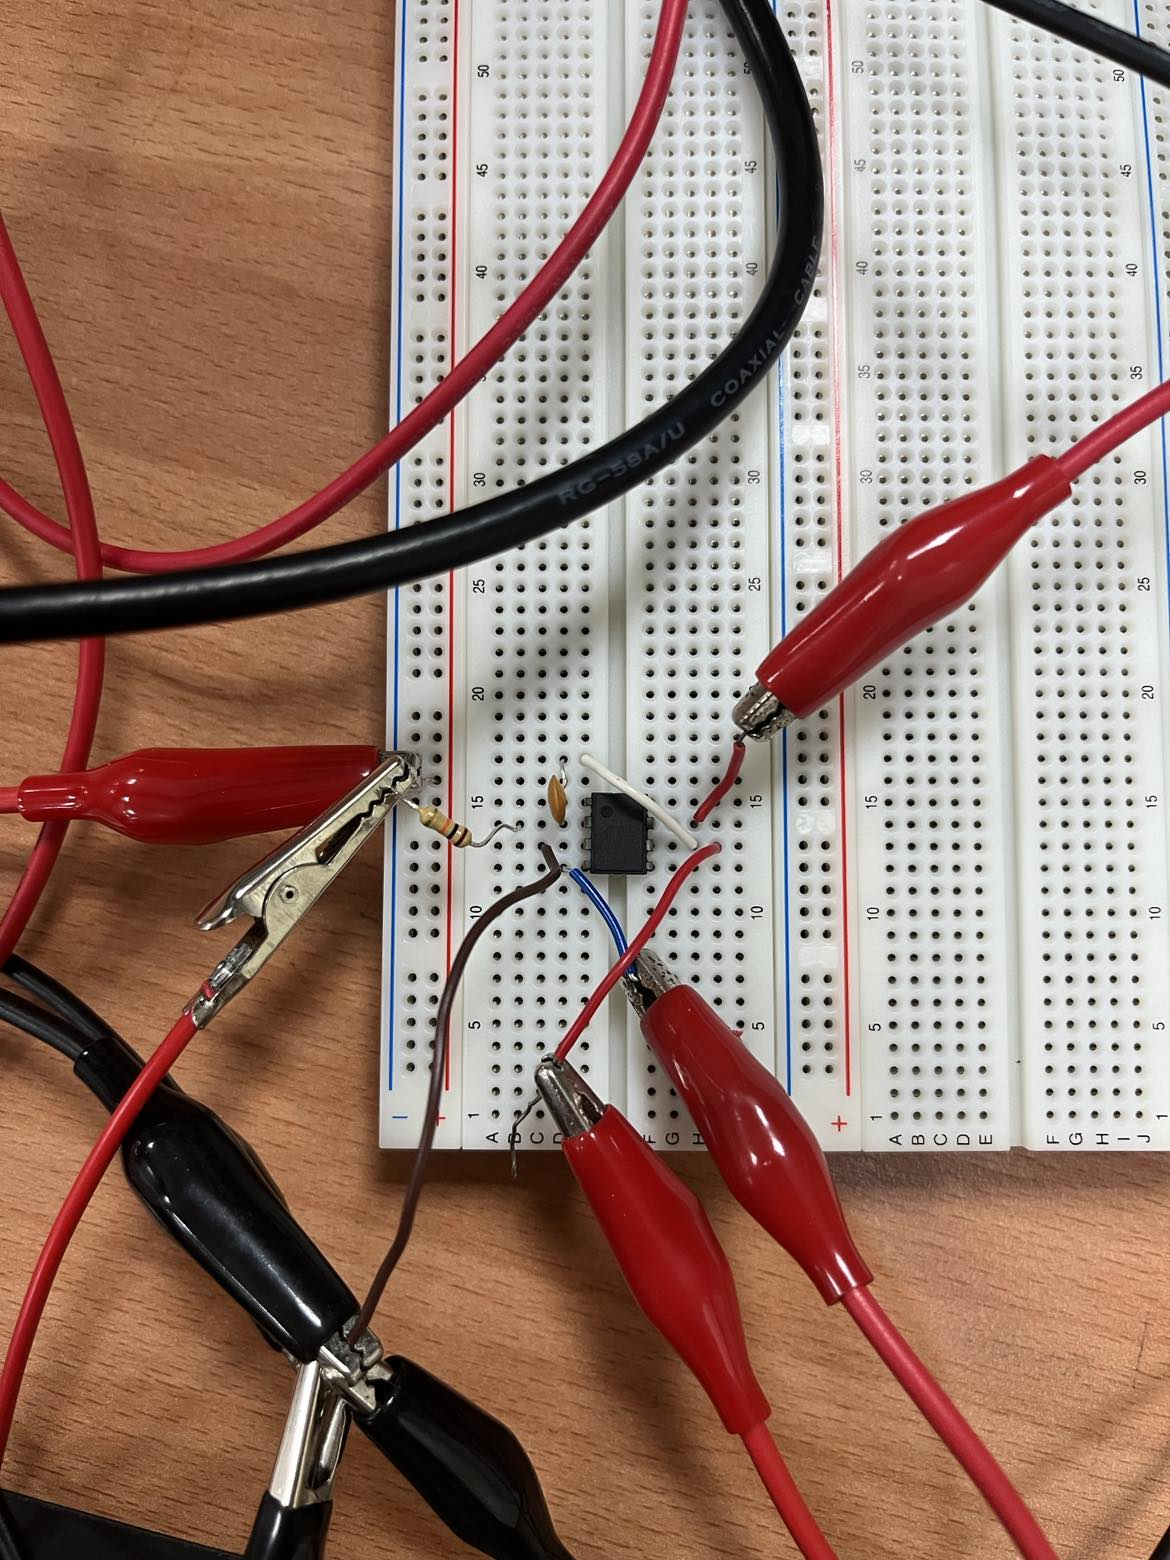
\includegraphics[width=\textwidth]{int_circuit.jpg}
        \caption{Integrator cicuit}
    \end{subfigure}
    ~
    \begin{subfigure}[b]{0.3\textwidth}
        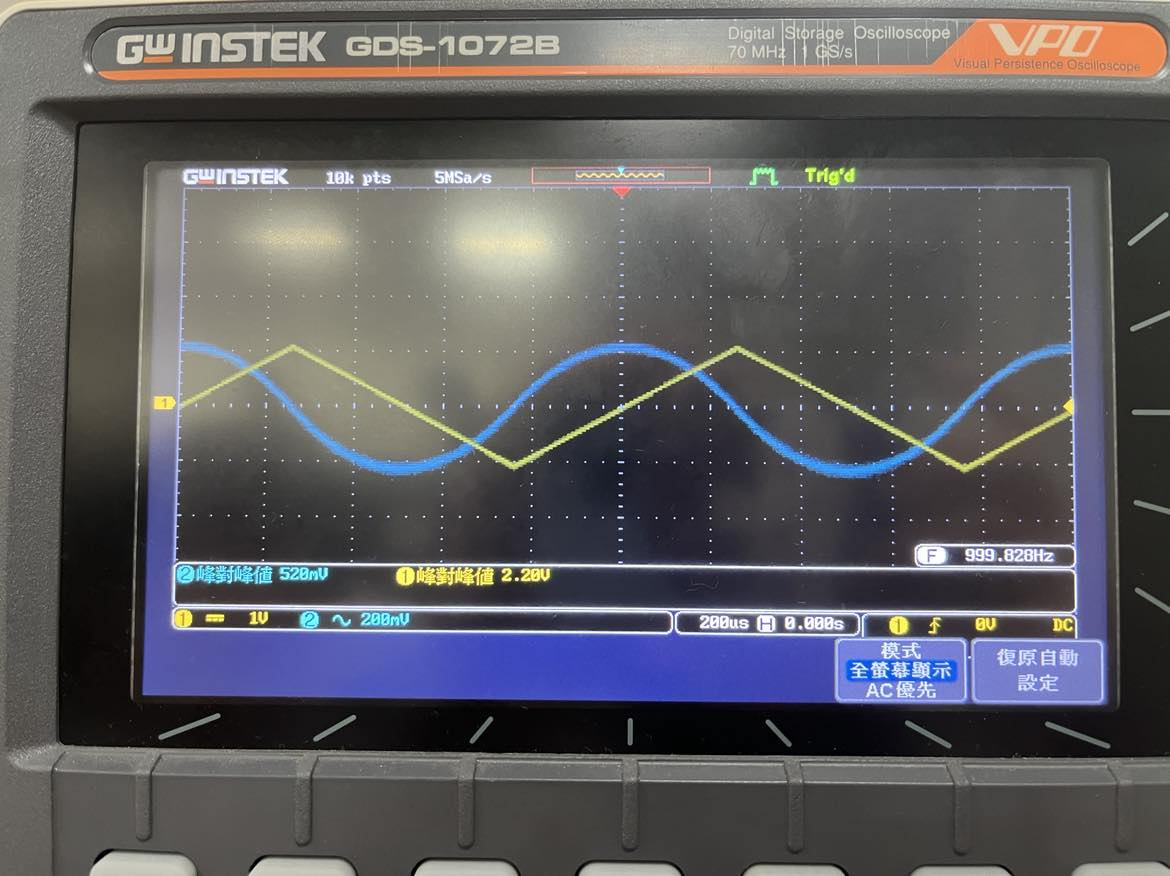
\includegraphics[width=\textwidth]{int_trig.jpg}
        \caption{Triangle wave input}
    \end{subfigure}

    \begin{subfigure}[b]{0.3\textwidth}
        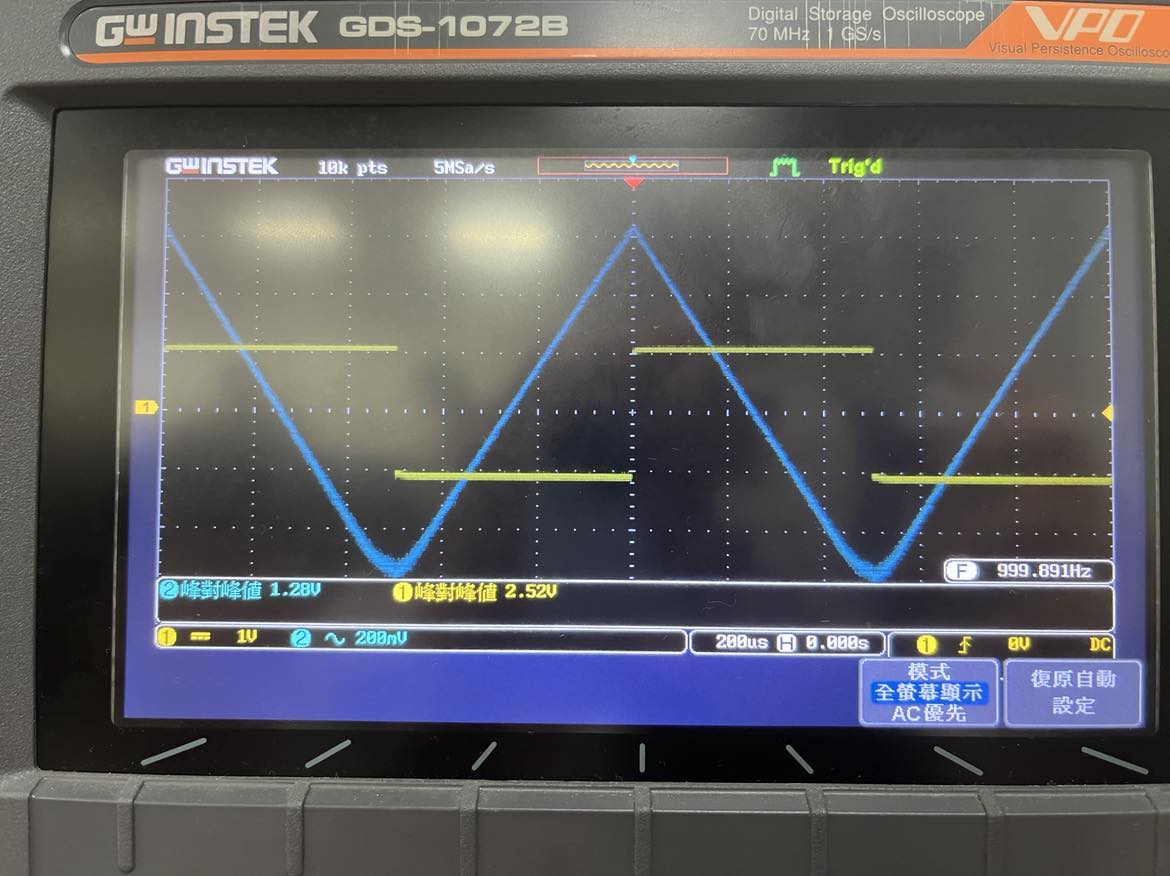
\includegraphics[width=\textwidth]{int_square.jpg}
        \caption{Square wave input}
    \end{subfigure}
    ~
    \begin{subfigure}[b]{0.3\textwidth}
        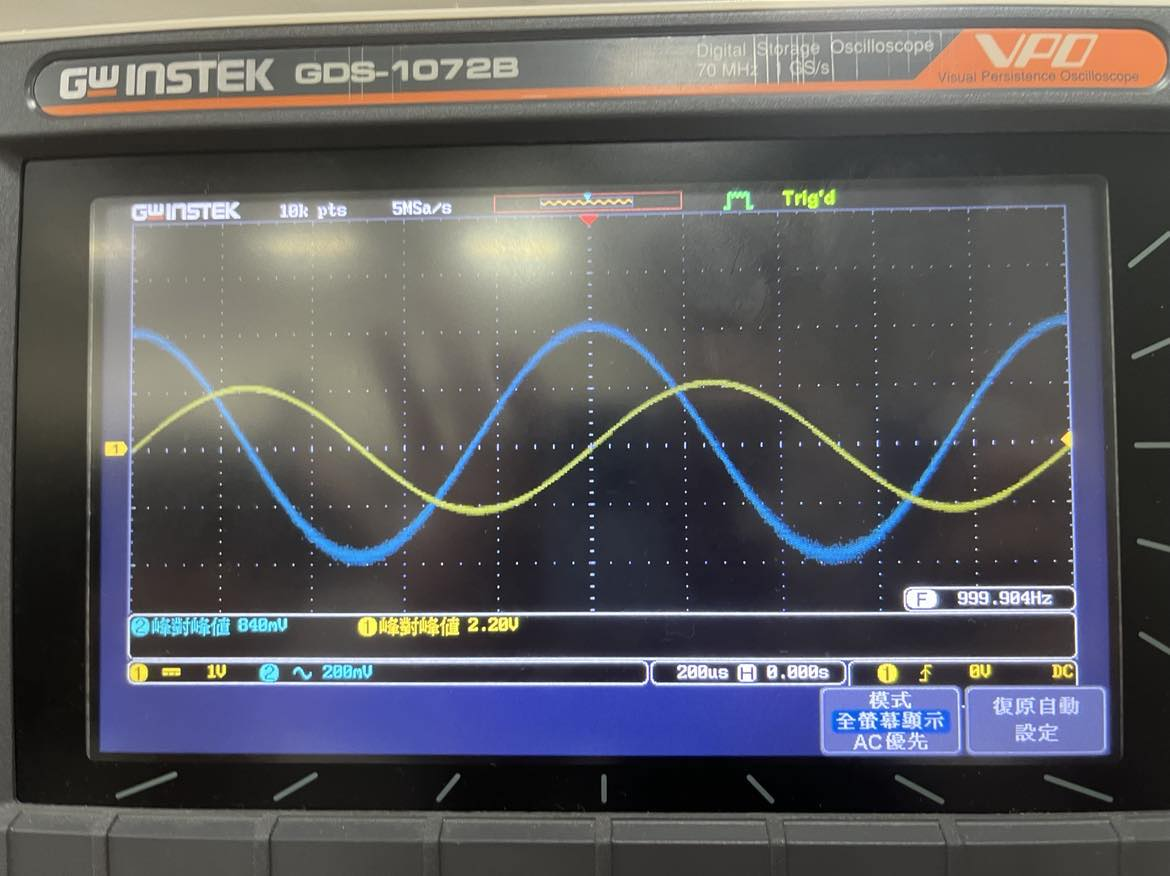
\includegraphics[width=\textwidth]{int_sin.jpg}
        \caption{Sinusoidal wave input}
    \end{subfigure}
\end{center}   
\end{figure}


%=========Non-Inverting OP-Amp Circuit=================
\section{Differentiator}


\begin{figure}[h]
    \begin{center}
    
        \begin{subfigure}[b]{0.2\textwidth}
            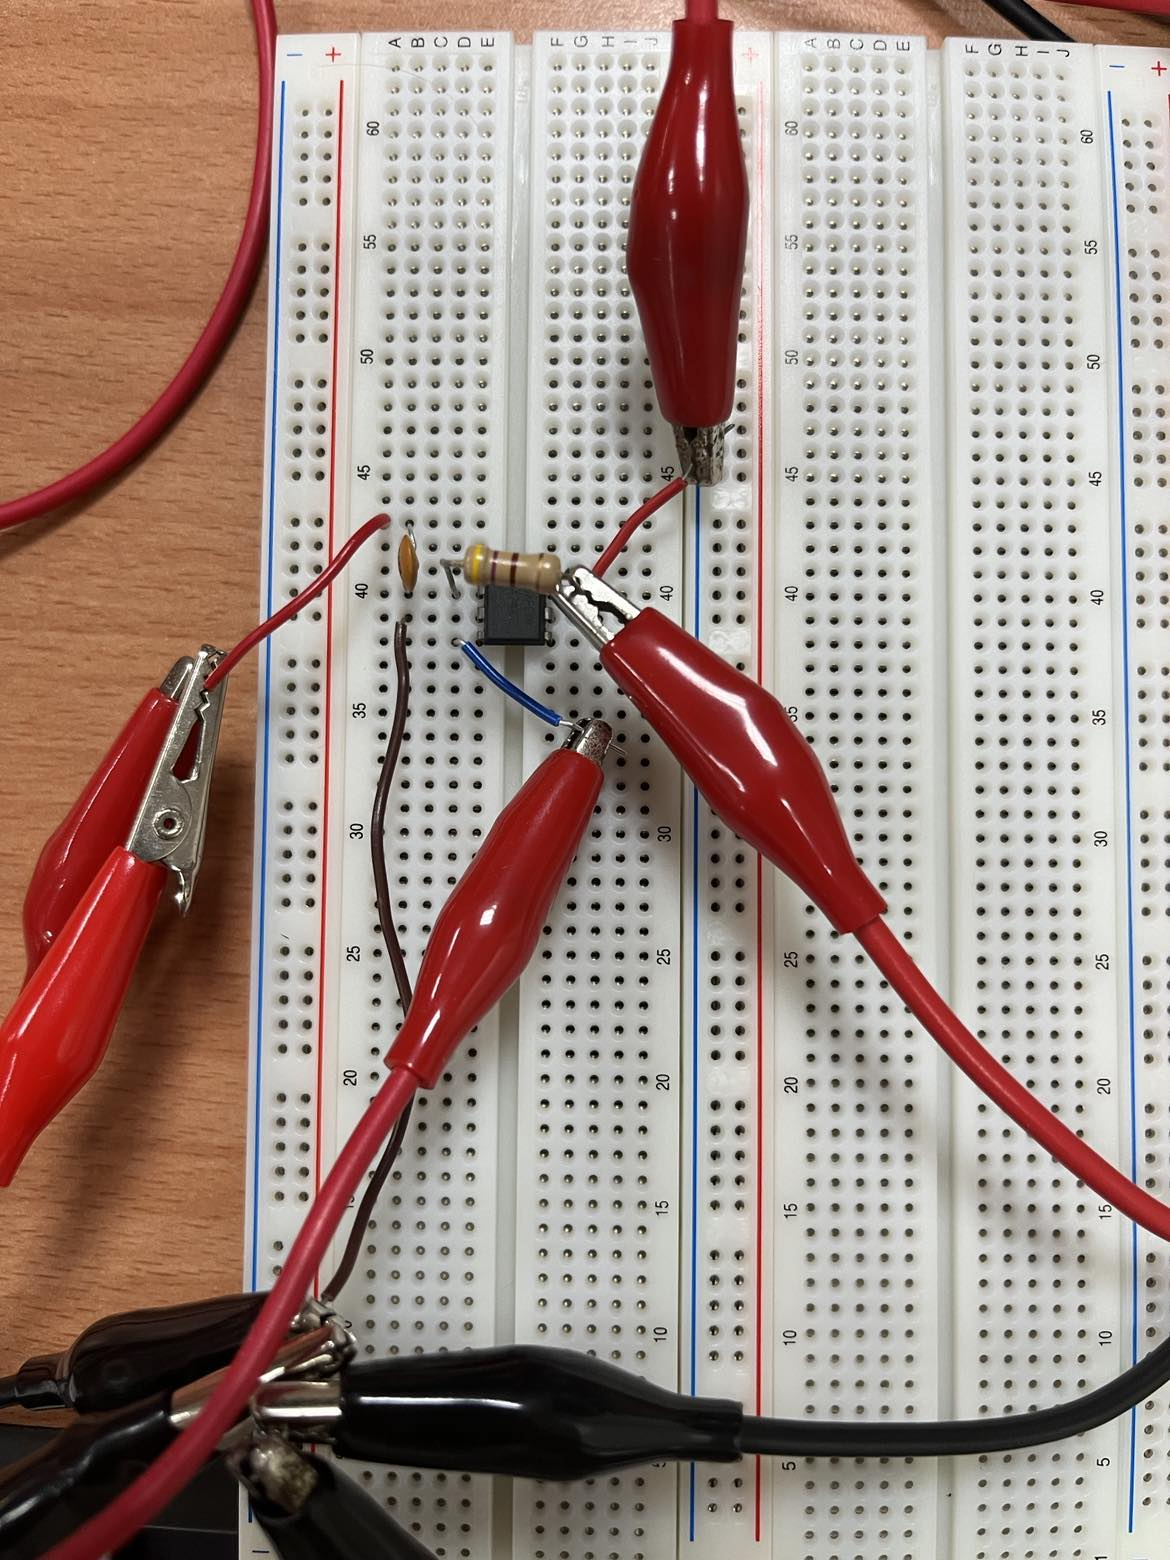
\includegraphics[width=\textwidth]{diff_circuit.jpg}
            \caption{Differentiator circuit}
        \end{subfigure}
        ~
        \begin{subfigure}[b]{0.3\textwidth}
            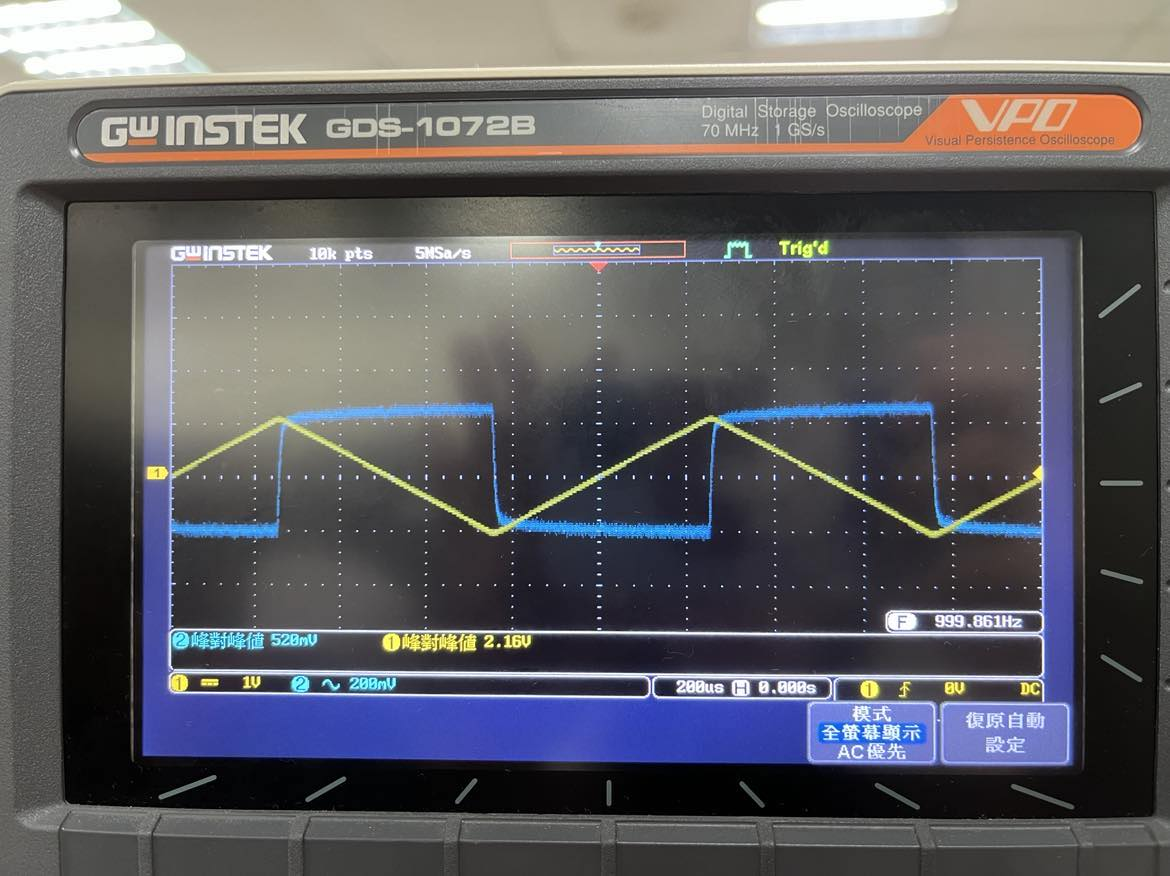
\includegraphics[width=\textwidth]{diff_trig.jpg}
            \caption{Triangle wave input}
        \end{subfigure}
    
        \begin{subfigure}[b]{0.3\textwidth}
            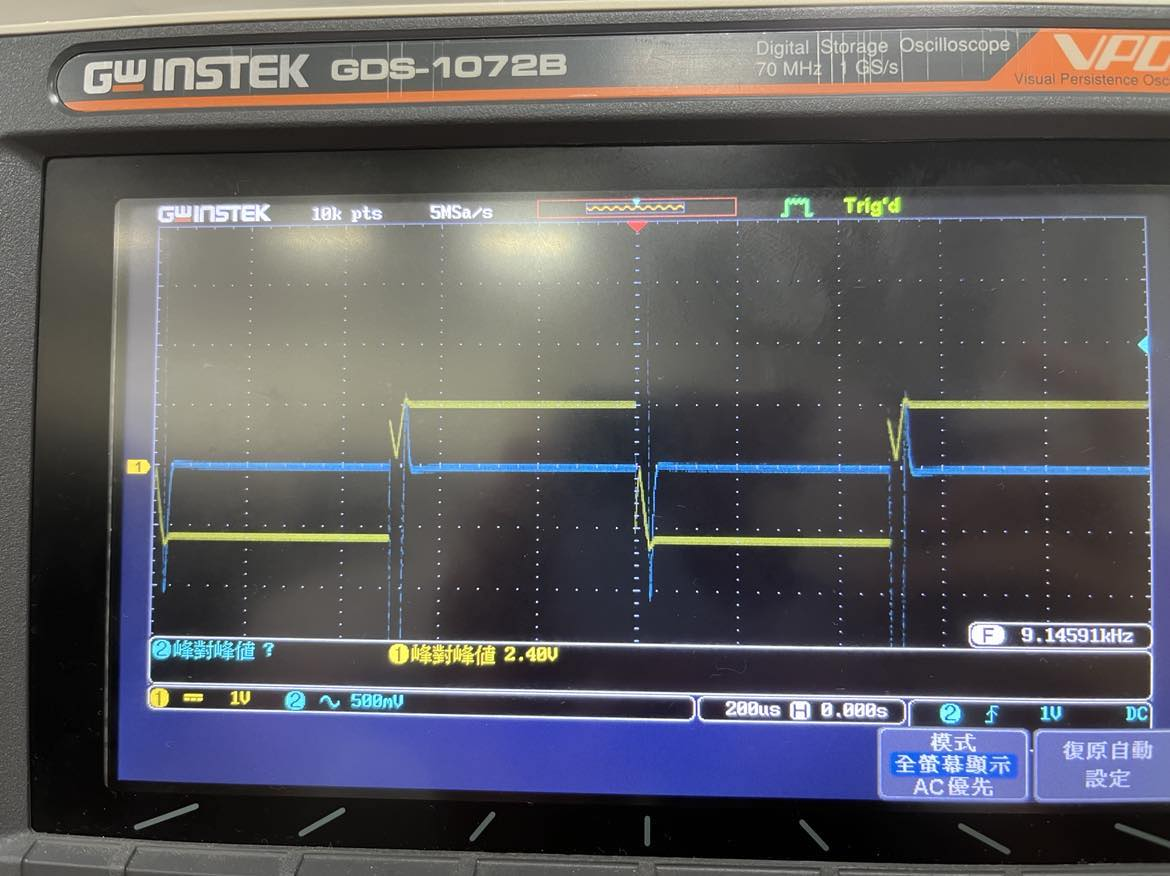
\includegraphics[width=\textwidth]{diff_square.jpg}
            \caption{Square wave input}
        \end{subfigure}
        ~
        \begin{subfigure}[b]{0.3\textwidth}
            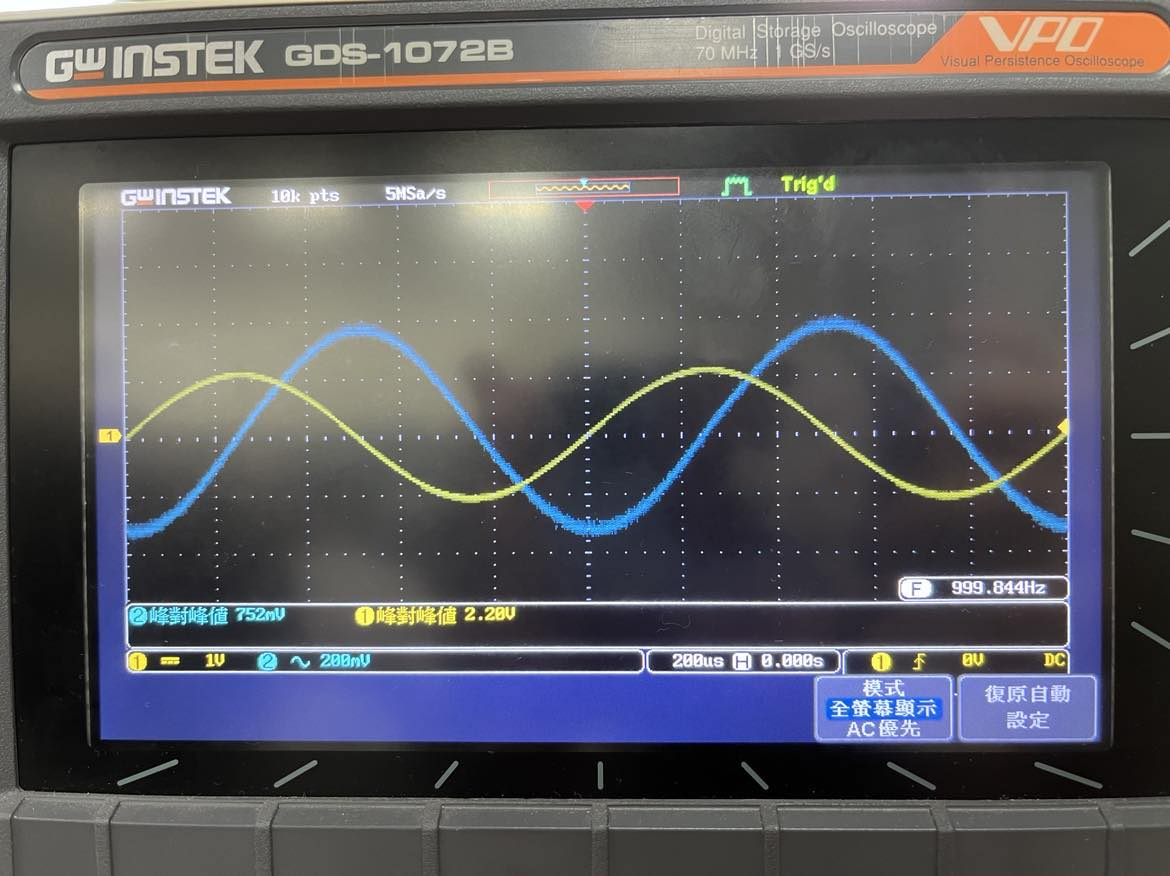
\includegraphics[width=\textwidth]{diff_sin.jpg}
            \caption{Sinusoidal wave input}
        \end{subfigure}
    \end{center}   
    \end{figure}
    

\end{CJK*}
\end{document}